% acmart 1.88 + recent hyperxmp fail ("hyperref must be loaded before hyperxmp"); skip hyperxmp (XMP metadata only)
\expandafter\def\csname ver@hyperxmp.sty\endcsname{}
\documentclass[sigconf]{acmart}
\settopmatter{printacmref=false, printccs=false, printfolios=true}
\renewcommand\footnotetextcopyrightpermission[1]{}


\usepackage{booktabs} % For formal tables
\usepackage{pgfplots}
\usepackage{enumitem}
\usepackage{array}
\pgfplotsset{compat=1.18}
\setlist{nosep,leftmargin=*}
\setlength{\emergencystretch}{1.5em}
\newcommand{\todo}[1]{\textcolor{red}{[TODO: #1]}}
\newcommand{\ver}[1]{\par\smallskip\noindent\textbf{#1.}\ }
\newcommand{\pa}{\textbf{(a)}~}\newcommand{\pb}{\textbf{(b)}~}\newcommand{\pc}{\textbf{(c)}~}\newcommand{\pd}{\textbf{(d)}~}
% (a) bottleneck observed, (b) hypothesis, (c) change made, (d) measured before/after result


\begin{document}
\title{Performance Engineering of a Spark Pipeline for NYC Yellow Taxi Analytics}
\subtitle{ComPar 2026/27 -- Project 1 -- Group \todo{number}}


\author{Diogo Oliveira}
\email{77474}

\author{Andr\'e Nunes}
\email{77077}


\begin{abstract}
This report describes how we profiled and optimised a Spark pipeline, written in Kotlin, that processes the 41\,M trips of the
2024 NYC Yellow Taxi data. The pipeline has five operations: cleaning, temporal demand, zone statistics with windows, fare
anomaly detection and trip-type classification. The baseline lost most of its time in repeated scans, in shuffles of whole trip
rows and in many small stages. We removed these problems one version at a time and measured each version. On an 8-core laptop
the full pipeline went from 63.5 to 28.1\,s (2.26$\times$). We also measured how the optimised pipeline behaves with more data,
with more cores and on a small Docker Spark cluster.
\end{abstract}

\keywords{Apache Spark, query optimisation, profiling, shuffle, scalability}


\maketitle
\pagestyle{plain} % no ACM conference running headers

% ============================================================================
\section{Introduction}
We use the 2024 NYC TLC Yellow Taxi trip records~\cite{tlc}: 12 monthly Parquet files (662\,MB compressed) with
41{,}169{,}720 trips and 19 columns, and the taxi zone lookup table with 265 rows.
We implemented the three mandatory operations, \textbf{M1} (ingestion and cleaning), \textbf{M2} (temporal demand per
borough, day of week and hour) and \textbf{M3} (monthly zone statistics with window functions), and two optional ones,
\textbf{O1} (fare anomaly detection with $\mu+3\sigma$ per zone and hour) and \textbf{O4} (trip-type classification).

From a performance point of view the workload is a large table that is reduced to a few thousand groups at most and joined
with a very small table. In principle each query should cost about one Parquet scan, and anything beyond that (extra scans,
shuffling full rows, spilling) comes from the way the query was written. We picked O1 and O4 because they both compute
statistics per bucket and then have to go back to every single trip. O1 does this with a window, which cannot pre-aggregate
before the shuffle, and O4 joins the bucket classes back to the full table. So both shuffle whole rows, something the
mandatory operations hardly do.

% ============================================================================
\section{Pipeline}
We wrote the pipeline in Kotlin with the Spark DataFrame API (we agreed this with the instructor instead of PySpark).
With the DataFrame API the compiler checks the query code, and inside an operation we can use Catalyst~\cite{sparksql}
queries together with normal JVM code when that is faster, as in the driver-side windows of M3~v3 and the columnar reader of
M1~v3. All operations implement the same \texttt{Analysis} interface and have numbered versions (\texttt{M1V0}\ldots\texttt{M1V3},
\texttt{O1V0}\ldots\texttt{O1V7}, \ldots). The version is a command-line option, so we can measure each change on its own against
the baseline. M1 returns the cleaned DataFrame without running it and the other operations read from it. We do not cache it,
because the 35\,M cleaned rows do not fit in a 4\,GB heap and each operation only reads the columns it uses.

Figure~\ref{fig:plan} has the physical plan of O1 before and after its most important change. We took it from the Spark event
log (it is the tree printed by \texttt{explain(mode="extended")}). In v0 all trips pass through
\texttt{Exchange hashpartitioning(PULocationID, hour)} and a \texttt{Sort} before the \texttt{Window}. In v3 the trips are only
read and looked up in a broadcast table, which comes from a partial \texttt{HashAggregate}.

\begin{figure}[t]
\centering\tiny
\begin{minipage}[t]{0.47\columnwidth}
\begin{verbatim}
WriteFiles
+- Sort
   +- Exchange
      +- HashAggregate
         +- Exchange
            +- HashAggregate
               +- BroadcastHashJoin
                  :- Project
                  :  +- Window
                  :     +- Sort
                  :        +- Exchange
                  :           +- Filter
                  :              +- Scan parquet
                  +- BroadcastExchange
                     +- Scan csv
\end{verbatim}
\end{minipage}\hfill
\begin{minipage}[t]{0.50\columnwidth}
\begin{verbatim}
WriteFiles
+- Sort
   +- Exchange
      +- HashAggregate
         +- Exchange
            +- HashAggregate
               +- BroadcastHashJoin
                  :- BroadcastHashJoin
                  :  :- Filter
                  :  :  +- Scan parquet
                  :  +- BroadcastExchange
                  :     +- HashAggregate
                  :        +- Exchange
                  :           +- HashAggregate
                  :              +- Scan parquet
                  +- BroadcastExchange
                     +- Scan csv
\end{verbatim}
\end{minipage}
\caption{Physical plan of O1 (Project nodes omitted): baseline with a Window over shuffled trips (left),
v3 with a broadcast of the per-bucket statistics (right).}
\label{fig:plan}
\end{figure}

% ============================================================================
\section{Profiling and Baseline}
\textbf{Setup.} Lenovo 83JX laptop: Intel Core Ultra 7 256V (8 cores / 8 threads, 2.2\,GHz base, 12\,MB L3), 16\,GB LPDDR5X-8533,
1\,TB NVMe SSD, Windows 11 (Balanced power plan). Temurin JDK 17.0.20, Kotlin 2.0.21, Spark 3.5.3 (Scala 2.12), Hadoop client 3.3.4.
Spark runs in \texttt{local[*]} (8 task slots) with \texttt{-Xmx4g}. The only settings we changed are AQE on (already the
default in 3.5) and the console progress bar off.
\textbf{Cluster.} We used the Spark standalone cluster from the course (\texttt{docker/docker-compose.yml}, image
\texttt{spark:python3}, which has Spark 4.2.0, Scala 2.13 and OpenJDK 21) in Docker Desktop on the same laptop. It has one
master and 1, 2 or 3 workers, each with 2 cores and 2\,GB (executors of 2\,GB). The Docker VM gets the 8 CPUs and 8\,GB. We
submit with \texttt{spark-submit -{}-deploy-mode client -{}-driver-memory 2g} from inside the master container, so the driver
runs there. The jar, the data and the output folder are mounted from Windows into every container. The script is
\texttt{scripts/cluster\_bench/cluster\_matrix.sh} and the README has the exact steps.

\textbf{Methodology.} Every configuration runs three times, each time in a new JVM so that no cache or JIT state carries over,
and we change the order of the 27 configurations in every round. We report the median and the min--max range. Each analytical
operation runs after M1~v3, and we only count its own time. The metrics come from our profiler, which reads the Spark REST
API~\cite{spark} (stages, tasks, CPU, GC, input, shuffle and spill per operation). We compared the output of every version with
the baseline and they are the same unless we say otherwise. \texttt{scripts/local\_bench/matrix.sh} and \texttt{analyze.sh}
rerun everything.

\begin{table}[t]
\centering\small\setlength{\tabcolsep}{3.2pt}
\caption{Baseline: full pipeline with every operation at v0 (median of 3; range of the total 62.2--65.8\,s).}
\label{tab:baseline}
\begin{tabular}{lrrrrrr}
\toprule
Op & wall (s) & stages & tasks & input & shuffle R/W & spill \\
   &          &        &       & (MB)  & (MB)        & (MB)  \\
\midrule
M1 & 11.53 & 10 & 76  & 1090 & 0.0 / 0.0     & 0    \\
M2 & 8.36  & 11 & 55  & 551  & 1.4 / 0.7     & 0    \\
M3 & 14.23 & 22 & 110 & 1101 & 1.3 / 1.3     & 0    \\
O1 & 13.25 & 14 & 101 & 556  & 423.9 / 423.9 & 1719 \\
O4 & 16.17 & 9  & 82  & 1173 & 584.9 / 584.9 & 0    \\
\midrule
Total & \textbf{63.54} & & & & & \\
\bottomrule
\end{tabular}
\end{table}

\textbf{What we found} (Table~\ref{tab:baseline}):
\begin{itemize}
\item \emph{Repeated scans.} M1 reads the data three times (two \texttt{count()} calls plus the per-year statistics), 1.09\,GB of
input for a 541\,MB projection. M3 reads it twice, because \texttt{show()} and \texttt{count()} are two actions and nothing is cached.
\item \emph{Shuffling whole rows.} The window of O1 over (zone, hour) sends all 35\,M trips through an Exchange: 424\,MB of
shuffle, 1.7\,GB spilled and 2.1\,GB of peak execution memory. O4 shuffles 585\,MB to join the bucket classes back to the trips.
\item \emph{Many small stages.} After the aggregation M3 only has about 3{,}000 rows, but each window adds another Exchange and
Sort (22 stages in total).
\item \emph{Little to gain.} M2 only shuffles 1.4\,MB, so its plan was already close to one scan.
\end{itemize}
As a lower bound, just decoding the Parquet columns we need takes about 3.1\,s with the 8 cores.

\textbf{Cluster baseline and skew.} With 2 workers (4 cores) the baseline takes 92.8\,s on the Docker cluster
(Table~\ref{tab:cluster}). Looking at the stages (task time, median run) we see the same picture as on the laptop. The biggest
stages are the scans of M1 (20.0 and 14.5\,s), M2 (26.3\,s) and M3 (28.2 and 25.4\,s), the stage of O1 that writes the shuffle
(27.0\,s, 423\,MB) and the window stage after it (58.5\,s, 342\,MB spilled to disk), and the stage of O4 that writes 583\,MB of
shuffle (46.1\,s). We did not find skew. The slowest task is at most 1.23$\times$ the median (the O1 window stage; 1.12$\times$
on the laptop), nowhere near 10$\times$. Each scan task reads one file and the shuffle keys have thousands of values, so the
work is spread evenly.

% ============================================================================
\section{Optimisation Study}
The times in this section come from the isolated runs (the operation after M1~v3), median of 3. Differences below about
5--7\,\% are inside the min--max range, so we count them as no change.

\subsection{M1: one scan and a direct columnar reader}
\ver{M1 v1: one scan}
\pa The baseline reads the data three times (1.09\,GB of input, 10 stages, 38.5\,s of CPU) and casts every column of every row.
\pb We expected that all counters could come out of a single pass, and the 2024 files already have the right types. \pc So v1
computes the total, the five criteria and the number of valid rows in one aggregation, checks the schema once and only casts
columns with the wrong type (none in 2024). \pd The time went from 11.27 to 5.65\,s (1.99$\times$), with input
1090\,$\rightarrow$\,539\,MB and CPU 38.5\,$\rightarrow$\,10.6\,s. This version also fixed a bug in the baseline: the cast of
\texttt{timestamp\_ntz} used the Lisbon time zone of the session, which moved trips inside the 31~March DST gap and dropped
493 valid trips.

\ver{M1 v2: bitmask per row}
\pa In v1 seven conditional sums each evaluate their own condition on every row. \pb If each row becomes one integer with a bit per
criterion, the aggregation should be cheaper. \pc v2 counts per (year, bitmask), which gives a few dozen groups, and the driver
computes all counters from them. \pd The time went from 5.65 to 5.22\,s (1.08$\times$).

\ver{M1 v3: direct columnar reader}
\pa Spark still turns every column batch into rows and then shuffles, while the only cost we really need is decoding Parquet.
\pb Reading the column vectors ourselves should avoid both. \pc In v3 each task reads the column batches of one file, computes the
bitmasks in simple loops and counts per (day, mask) in an array, and the driver adds up the 12 arrays. \pd The time went from 5.22
to 3.14\,s (1.66$\times$, 3.59$\times$ against v0), with 2 stages, 13 tasks and no shuffle, which is about the time it takes to
decode the columns.

\subsection{M2: little room above the scan}
M2 was already limited by the scan (1.4\,MB of shuffle), and every version takes between 5.8 and 6.9\,s.

\ver{M2 v1: projection and broadcast}
\pa The baseline reads 551\,MB for a query that needs five columns and joins the zone table. \pb Selecting the columns ourselves and
forcing a broadcast should read less and make the join cheaper. \pc v1 does exactly that. \pd The plan metrics did not change (input, stages, shuffle). The
time went from 6.21 to 5.79\,s here, but in our three batteries the gain was 1.00, 1.02 and 1.07$\times$: Catalyst was already
pruning the columns and broadcasting the 12\,KB table, which is under the 10\,MB threshold.

\ver{M2 v2: no global sort}
\pa The \texttt{orderBy} before the partitioned write adds a shuffle with range partitioning (11 stages), but
\pb \texttt{partitionBy(borough)} only needs the rows grouped by borough. \pc v2 uses \texttt{repartition(borough)} instead. \pd Stages
11\,$\rightarrow$\,9, shuffle 1.4\,$\rightarrow$\,0.7\,MB and 5.98\,s, which is within noise.

\ver{M2 v3: aggregate before the join (rejected)}
\pa The join with the zone table is applied to all 35\,M trips before the aggregation. \pb Aggregating first should shrink the input of the join. \pc v3 aggregates by (zone, day, hour)
first, then joins and aggregates by borough. \pd It got \emph{slower} (6.92\,s, 8.8\,MB of shuffle), because there are 37$\times$
more zone groups than borough groups, so we dropped it.

\ver{M2 v4: no join}
\pa v2 still has the join and a second aggregation, with 217\,MB of peak execution memory. \pb Zone$\rightarrow$borough is a map with
265 entries, so it does not need a join. \pc v4 builds the map on the driver, packs (borough, day, hour) into an 11-bit integer and
aggregates once. \pd 5.88\,s (1.06$\times$), no join, and peak memory 217\,$\rightarrow$\,17\,MB.

\ver{M2 v5--v7: less work per row}
\pa v4 evaluates a chain of \texttt{CASE WHEN} and \texttt{unix\_timestamp} on every row. \pb Less work per row and fewer small stages should help. \pc v5 uses an array lookup and divides the
duration once per group, v6 writes with \texttt{coalesce(1)} and v7 reads the CSV on the driver. \pd v6 and v7 have 6 and 5 stages,
but they were 9--12\,\% slower than v4 and used 23\,\% more CPU. In the end v1, v2 and v4 are all within noise of each other.

\subsection{M3: one scan, integer keys, windows on the driver}
\ver{M3 v1: cache the result}
\pa \texttt{show()} and \texttt{count()} each read and aggregate the trips again (1.08\,GB of input). \pb If we cache the small final
table the second action costs almost nothing. \pc v1 caches the result (about 3{,}000 rows) and broadcasts the zone table. \pd 12.52
$\rightarrow$\,10.09\,s (1.24$\times$), half the input and CPU 46.4\,$\rightarrow$\,27.9\,s. One side effect: the cached result
keeps the 200 shuffle partitions, because AQE does not merge them, and the tasks went from 112 to 734.

\ver{M3 v2: integer keys}
\pa \texttt{date\_format} creates a string for each of the 35\,M rows, and the grouping key contains strings. \pb If we group by integers
and only join after the aggregation, that work is done on 3{,}000 rows instead. \pc v2 groups by (\texttt{PULocationID},
$\text{year}\cdot100+\text{month}$) and joins and formats afterwards. \pd 10.09\,$\rightarrow$\,7.69\,s (1.31$\times$), CPU
27.9\,$\rightarrow$\,15.8\,s.

\ver{M3 v3: windows on the driver}
\pa The windows still need their own Exchange and Sort, for only 3{,}000 rows (38 stages). \pb With so few rows a loop on the driver
should be cheaper than scheduling more stages. \pc v3 collects the aggregated rows and computes the rank, the 3-month rolling share
and the deviation flag (Welford~\cite{welford}) in Kotlin. \pd 7.69\,$\rightarrow$\,4.71\,s (1.63$\times$, 2.66$\times$ against v0),
6 stages, 28 tasks and 0.3\,MB of shuffle. While testing this we noticed that the original flag could never be true: if the
current month is inside the 3-row frame, $|x-\bar{x}|/s \le 1.155 < 1.5$. All versions now use the three \emph{previous} months.

\subsection{O1: from a window to a broadcast}
\ver{O1 v1 and v2: projection and broadcast}
\pa The baseline keeps all columns through several projections and joins the zone table. \pb One projection and a forced broadcast
should move less data and make the join cheaper. \pc v1 uses a single \texttt{select} and v2 adds \texttt{broadcast(zones)}. \pd The times were 12.90, 12.62 and 12.55\,s with the same plan
metrics: Catalyst was already pruning the columns, merging the projections and broadcasting the zone table.

\ver{O1 v3: aggregation instead of a window}
\pa A window cannot combine on the map side, so every trip is shuffled (424\,MB) and the largest buckets spill (1.7\,GB). \pb But
$\mu$ and $\sigma$ per bucket are just an aggregation with at most 263$\times$24 groups. \pc v3 uses \texttt{groupBy(zone, hour)},
which aggregates partially before the shuffle, and broadcasts the 6{,}312 thresholds back to the trips.
\pd 12.55\,$\rightarrow$\,8.67\,s (1.45$\times$), shuffle 424\,$\rightarrow$\,2.9\,MB, no spill, peak memory
2.1\,GB\,$\rightarrow$\,205\,MB and CPU 51.2\,$\rightarrow$\,29.0\,s. The price is a second scan (input 546\,$\rightarrow$\,1087\,MB).

\ver{O1 v4 and v5: integer keys and an array instead of the join}
\pa The broadcast hash join still hashes and probes 35\,M rows, and the aggregation carries strings. \pb Integer keys and reading
straight from an array should be cheaper. \pc v4 uses a 14-bit bucket key and an 8-bit rate key with the borough resolved on the
driver, and v5 collects the thresholds into a
67\,KB array indexed by the key (\texttt{element\_at}), so no join is left. \pd v4: 8.83\,s (0.98$\times$, within noise), but peak memory 205\,$\rightarrow$\,34\,MB. v5: 7.96\,s (1.11$\times$), CPU 29.7\,$\rightarrow$\,24.0\,s.

\ver{O1 v6 and v7: less arithmetic per trip}
\pa v5 updates a floating-point average for the anomaly rate on every trip and converts every fare to per-km in both scans. \pb The
rate can be computed from two integer counts, and $x>\mu+3\sigma$ does not change if everything is multiplied by $1/1.609$.
\pc v6 uses a single aggregation with integer counters and computes the rate only on the 84 output rows; v7 computes the thresholds
and the comparison in fare per mile. \pd They took 7.88 and 7.95\,s, CPU 24.0\,$\rightarrow$\,22.2\,s, which is within noise: at
this point O1 costs about its two scans (1.64$\times$ against v0).

\subsection{O4}
We only have the baseline (13.49\,s, 585\,MB of shuffle, 59\,s of CPU, the most of any operation). Its metrics look like
those of O1~v0, so the same fix should work: broadcast or look up the $\le$6{,}312 bucket classes in an array. \todo{O4 v1}

\begin{table}[t]
\centering\footnotesize\setlength{\tabcolsep}{2.6pt}
\caption{Summary of all optimisations (median of 3 isolated runs; speedups as ratios of wall time).}
\label{tab:summary}
\begin{tabular}{llrrrl}
\toprule
Op & ver & wall (s) & vs v0 & vs prev & main metric change \\
\midrule
M1 & v0 & 11.27 & 1.00 & -- & 3 scans, 1090\,MB in \\
   & v1 & 5.65 & 1.99 & 1.99 & 1 scan, 539\,MB in \\
   & v2 & 5.22 & 2.16 & 1.08 & CPU 10.6$\rightarrow$12.1\,s \\
   & v3 & 3.14 & 3.59 & 1.66 & 2 stages, no shuffle \\
\midrule
M2 & v0 & 6.21 & 1.00 & -- & 11 stages \\
   & v1 & 5.79 & 1.07 & 1.07 & same plan metrics \\
   & v2 & 5.98 & 1.04 & 0.97 & 9 stages \\
   & v3 & 6.92 & 0.90 & 0.86 & shuffle 8.8\,MB \\
   & v4 & 5.88 & 1.06 & 1.18 & peak 217$\rightarrow$17\,MB \\
   & v5 & 6.60 & 0.94 & 0.89 & CPU +23\,\% \\
   & v6 & 6.57 & 0.95 & 1.00 & 6 stages \\
   & v7 & 6.41 & 0.97 & 1.02 & 5 stages \\
\midrule
M3 & v0 & 12.52 & 1.00 & -- & 2 scans, 24 stages \\
   & v1 & 10.09 & 1.24 & 1.24 & 1 scan \\
   & v2 & 7.69 & 1.63 & 1.31 & CPU 27.9$\rightarrow$15.8\,s \\
   & v3 & 4.71 & 2.66 & 1.63 & 6 stages, 0.3\,MB shuffle \\
\midrule
O1 & v0 & 12.90 & 1.00 & -- & 424\,MB shuffle, 1.7\,GB spill \\
   & v1 & 12.62 & 1.02 & 1.02 & same plan metrics \\
   & v2 & 12.55 & 1.03 & 1.01 & same plan metrics \\
   & v3 & 8.67 & 1.49 & 1.45 & 2.9\,MB shuffle, no spill \\
   & v4 & 8.83 & 1.46 & 0.98 & peak 205$\rightarrow$34\,MB \\
   & v5 & 7.96 & 1.62 & 1.11 & no join, CPU 24.0\,s \\
   & v6 & 7.88 & 1.64 & 1.01 & CPU 22.2\,s \\
   & v7 & 7.95 & 1.62 & 0.99 & no change \\
\midrule
O4 & v0 & 13.49 & 1.00 & -- & 585\,MB shuffle \\
\midrule
All & v0$\rightarrow$best & 63.54$\rightarrow$28.06 & 2.26 & & full pipeline \\
\bottomrule
\end{tabular}
\end{table}

Table~\ref{tab:summary} lists all versions. Running the full pipeline with the optimised versions
(\texttt{-{}-m1 v3 -{}-m2 v7 -{}-m3 v3 -{}-o1 v7 -{}-o4 v0}) takes 28.06\,s instead of 63.54\,s (2.26$\times$).

% ============================================================================
\section{Analysis}
Unless we say otherwise, these runs use the optimised pipeline (ALL\_best), three times each with a new JVM (local) or a
new \texttt{spark-submit} (cluster), in rotated order, and we give the median. The local runs were done in a different battery
from Table~\ref{tab:summary}, so absolute times can differ by up to about 15\,\%.

\begin{figure}[t]
\centering
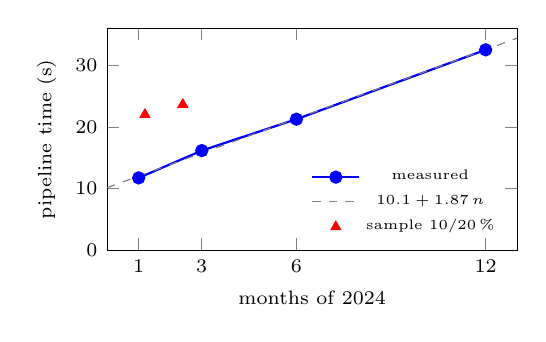
\begin{tikzpicture}
\begin{axis}[width=0.56\columnwidth,height=4.4cm,xlabel={months of 2024},ylabel={pipeline time (s)},
  xmin=0,xmax=13,ymin=0,ymax=36,xtick={1,3,6,12},label style={font=\scriptsize},tick label style={font=\scriptsize},
  legend style={font=\tiny,at={(0.98,0.02)},anchor=south east,draw=none,fill=none}]
\addplot[mark=*,thick,blue] coordinates {(1,11.72)(3,16.15)(6,21.24)(12,32.50)};
\addplot[dashed,gray,domain=0:13] {10.14+1.866*x};
\addplot[only marks,mark=triangle*,red] coordinates {(1.2,22.00)(2.4,23.63)};
\legend{measured,$10.1+1.87\,n$,sample 10/20\,\%}
\end{axis}
\end{tikzpicture}\hfill
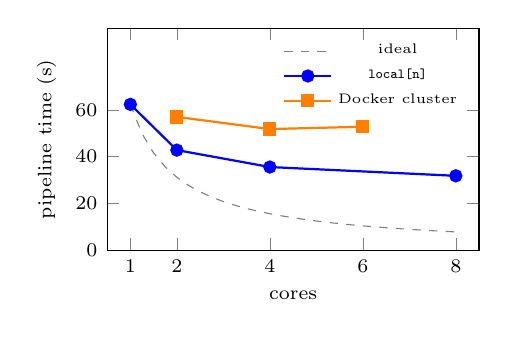
\begin{tikzpicture}
\begin{axis}[width=0.52\columnwidth,height=4.4cm,xlabel={cores},ylabel={pipeline time (s)},
  xmin=0.5,xmax=8.5,ymin=0,ymax=95,xtick={1,2,4,6,8},ytick={0,20,40,60},label style={font=\scriptsize},
  tick label style={font=\scriptsize},legend style={font=\tiny,at={(0.98,0.98)},anchor=north east,draw=none,fill=none}]
\addplot[dashed,gray,domain=1:8,samples=29] {62.4/x};
\addplot[mark=*,thick,blue] coordinates {(1,62.40)(2,42.83)(4,35.58)(8,31.82)};
\addplot[mark=square*,thick,orange] coordinates {(2,57.04)(4,51.83)(6,52.83)};
\legend{ideal,\texttt{local[n]},Docker cluster}
\end{axis}
\end{tikzpicture}
\caption{Scalability of the optimised pipeline. Left: time vs.\ number of months (sampled runs drawn at 10/20\,\%
of 12 months). Right: time vs.\ cores on the 12 months, locally and on the Docker cluster with 1--3 workers of 2 cores.}
\label{fig:scaling}
\end{figure}

\textbf{Dataset scale.} With 1, 3, 6 and 12 months (3.0\,M to 41.2\,M trips) the pipeline takes 11.7, 16.2, 21.2 and 32.5\,s
(for 12 months this is the median of six runs, 30.8--43.0\,s). A least-squares fit gives
$10.1\,\text{s} + 1.87\,\text{s}$ per month (Figure~\ref{fig:scaling}). So the time grows \emph{sub-linearly}: 12$\times$ more
data takes 2.8$\times$ more time. About 10\,s do not depend on the input (starting the JVM, jobs and stages, work on the driver,
the lookup table, the small final stages), and only the part that scans the data grows linearly.
Sampling does not help much. \texttt{-{}-sample 0.1} still takes 22.0\,s (68\,\% of the full run) and \texttt{-{}-sample 0.2}
takes 23.6\,s. The sample is taken \emph{after} reading, so every Parquet file is still decoded (M2 still reads 539\,MB), and
M1~v3 has to fall back to v2 when sampling (5.7 instead of 3.1\,s). Only O4, which shuffles a lot, really gains
(12.0\,$\rightarrow$\,5.0\,s, shuffle 585\,$\rightarrow$\,62\,MB).

\textbf{Number of cores.} On the 12 months, \texttt{local[1]}, \texttt{[2]}, \texttt{[4]} and \texttt{[8]} take 62.4, 42.8,
35.6 and 31.8\,s. That is a speedup of 1.46, 1.75 and 1.96 and an efficiency of 73\,\%, 44\,\% and 25\,\%. If we fit Amdahl's law
to these points the serial fraction is about 0.4. We see three reasons for this. First, the fixed cost on the driver and in
scheduling stays the same with more cores. Second, the scans have one task per file, so 12--13 tasks for 8 slots, and in the
second wave half of the cores have nothing to do. Third, the Core Ultra 7 256V has 4 performance cores and 4 slower efficiency
cores, so going from 4 to 8 cores only gives 1.12$\times$, and all cores share the memory bandwidth that Parquet decoding needs.
O4, which uses the most CPU and shuffle, scales best (2.45$\times$). M2, which is mostly the scan and one tiny aggregation,
scales worst (1.70$\times$).

\begin{table}[t]
\caption{Docker standalone cluster, 12 months (median of 3 \texttt{spark-submit}s; range of the total in brackets).}
\label{tab:cluster}
\centering\footnotesize\setlength{\tabcolsep}{2.4pt}
\begin{tabular}{lrrrrrrr}
\toprule
config & cores & total (s) & M1 & M2 & M3 & O1 & O4 \\
\midrule
1 worker, best & 2 & 57.0 {\tiny(55.9--61.2)} & 6.2 & 12.4 & 5.2 & 12.3 & 21.4 \\
2 workers, v0 & 4 & 92.8 {\tiny(91.6--113.9)} & 15.8 & 11.3 & 19.2 & 25.4 & 21.8 \\
2 workers, best & 4 & 51.8 {\tiny(46.5--57.5)} & 7.7 & 11.2 & 4.7 & 9.9 & 18.5 \\
\quad sample 10\,\% & 4 & 37.2 {\tiny(34.1--38.8)} & 9.6 & 7.2 & 3.9 & 6.9 & 7.6 \\
\quad sample 20\,\% & 4 & 35.7 {\tiny(34.3--53.1)} & 9.2 & 6.6 & 3.4 & 7.7 & 9.0 \\
3 workers, best & 6 & 52.8 {\tiny(49.0--54.2)} & 6.5 & 12.3 & 4.9 & 10.1 & 16.8 \\
\bottomrule
\end{tabular}
\end{table}

\textbf{Docker cluster} (Table~\ref{tab:cluster}). All 18 runs finished without errors. With 2 workers the optimisations
bring the pipeline from 92.8 to 51.8\,s (1.79$\times$), and the versions rank the same way as on the laptop. M3 (4.1$\times$) and
O1 (2.6$\times$) gain more than locally, since their baselines pay more for shuffles and stages between executors (O1~v0 spills
2.6\,GB with 2\,GB executors). But adding workers barely helps: 57.0, 51.8 and 52.8\,s with 2, 4 and 6 cores (speedup 1.10 and
1.08, efficiency 55\,\% and 36\,\%), and 1 worker is 33\,\% slower than \texttt{local[2]} (42.8\,s). The executor CPU time for
the same work goes from 68\,s with 1 worker to 94\,s with 2 and 125\,s with 3. All workers are containers in the same VM, so the
6 executor cores, the driver and the master share the same 8 CPUs (4 of them efficiency cores), and every Parquet file is read
through the mount from Windows. Adding a worker here only adds competition for the same CPUs. O4, the operation with the big
shuffle, is the only one that keeps improving (21.4, 18.5 and 16.8\,s). Sampling behaves like on the laptop: 10\,\% of the data
still takes 72\,\% of the time (20\,\% is within noise of that), because the whole input is read anyway. O4 drops from 18.5 to
7.6\,s (shuffle 585\,$\rightarrow$\,61\,MB) and M1 gets slower (v3 falls back to v2 when sampling).

% ============================================================================
\section{Discussion}
\textbf{What is left.} After the optimisations each operation costs roughly its own scan. M1~v3 takes about the time to decode
the columns, and M2, M3 and O1 spend most of their time reading 0.5--1.1\,GB of Parquet. What remains is that every operation
reads the same files again. Materialising the cleaned data once would fix this, either with a cache on a cluster with enough
memory or by writing a narrower Parquet file. O4 still shuffles 585\,MB.

\textbf{Limitations.} Everything was measured on one laptop, with three runs per configuration. The Docker cluster runs on the
same CPUs and uses Spark 4.2 instead of 3.5, so it shows the overhead of running on a cluster but not what real extra machines
would give. We ran the whole matrix three times on the same laptop and got 58.0, 71.2 and 63.5\,s for the baseline and 26.3,
30.8 and 28.1\,s for the optimised pipeline (2.20, 2.31 and 2.26$\times$). The CPU time changed by the same amount, so we think
the processor frequency changed between batteries, and the versions ranked the same every time. We report the third battery.
On Windows without \texttt{winutils.exe} our benchmark uses a local file system that skips the Hadoop permission calls. This only
affects listing folders and writing, not reading or computing. The peak memory from the profiler is the sum of the task peaks in
a stage, so it is too high for stages with many tasks (M3~v1). The M1~v3 reader does not go through Spark's \texttt{FileScan}, so
Spark reports no input bytes for it.

\textbf{With more time} we would implement O4~v1, repeat the cluster tests on real machines (the DI cluster) and measure
how much it costs to materialise the output of M1.


% ============================================================================
\clearpage
\begin{acks}
We used Claude Code (Anthropic) during the project, mostly to help with research, with the code and with writing this
report. We ran and checked all the measurements ourselves.
\end{acks}

\section*{Individual contributions}
\begin{tabular}{@{}l>{\raggedright\arraybackslash}p{0.52\columnwidth}l@{}}
\toprule
Member & Work & \% \\
\midrule
Diogo Oliveira & M1, M3, benchmark, report \todo{confirm} & \todo{\%} \\
Andr\'e Nunes & M2, O1, profiler, Docker benchmark \todo{confirm} & \todo{\%} \\
\bottomrule
\end{tabular}


\bibliographystyle{acm}
\bibliography{refs}

\end{document}
